\chapter{ギャップ増幅補題} \label{chap:gap-amplification}

DinurによるPCP定理の証明は, 与えられた制約グラフの不満足値を段階的に増幅していくアプローチに基づく.
その中核を担うのがこのギャップ増幅補題であり, 制約グラフの不満足値を増幅できることを保証する補題である.
本チャプターはこの補題の証明を与える.

\section{主張}
ギャップ増幅補題は以下のように述べられる.

\begin{lemma}{ギャップ増幅補題}{gap-amplification-lemma}
  二つの定数$c>0,\alpha\in (0,1)$, アルファベット$\Sigma$, および以下の性質を満たす決定的多項式時間アルゴリズム$A$が存在する: 
  アルゴリズム$A$は制約グラフ$G=\ip{(V,E),\Sigma,\calC}$を入力として受け取り, 次の性質を満たす別の制約グラフ$G'=\ip{(V',E'),\Sigma,\calC'}$を出力する:
  \begin{itemize}
    \item $\size(G')\le c\cdot \size(G)$.
    \item $\UNSAT(G)=0$ならば$\UNSAT(G')=0$.
    \item $\UNSAT(G)>0$ならば$\UNSAT(G')\ge \min\{\alpha, 2\cdot \UNSAT(G)\}$.
  \end{itemize}
\end{lemma}

PCP定理(\cref{thm:PCP-CSP-theorem})の証明は, この補題を繰り返し適用することによって得られる.

\begin{proof}[\cref{lem:gap-amplification-lemma}の下での\cref{thm:PCP-CSP-theorem}の証明.]
  3彩色問題のインスタンスを入力として受け取り, その制約グラフを$G_0$とし, 頂点数を$n$とする.
  この制約グラフは単純グラフであるため, $\UNSAT(G_0)=0$もしくは$\UNSAT(G_0)\ge \frac{1}{n^2}$である.
  \cref{lem:gap-amplification-lemma}のアルゴリズムを$A$とし, 各$i=1,\dots,\ceil{2\log_2 n}$について, 制約グラフ$G_i$を
  $G_i = A(G_{i-1})$として定義し, 最終的に得られる制約グラフを$G'=G_{\ceil{2\log_2 n}}$とする.
  各$G_i$のサイズは$\size(G_i) \le c\cdot \size(G_{i-1})$であるため, $\size(G')\le c^{\ceil{2\log_2 n}}\cdot \size(G_0)=\size(G_0)^{O(1)}$である.
  従って$G'$は多項式時間で構成できる.

  また, 不満足値については, 以下のようになる:
  \begin{itemize}
  \item もしも$G_0$がYesインスタンスであるならば, 全ての$i$に対して$G_i$もYesインスタンスであり, 特に$\UNSAT(G')=0$である.
  \item もしも$G_0$がNoインスタンスであるならば, $\UNSAT(G_0)\ge \frac{1}{n^2}$かつ$\UNSAT(G_i)\ge \min\{\alpha, 2\cdot \UNSAT(G_0)\}$であるため, $\UNSAT(G')\ge \min\qty{\alpha, 2^{2\log_2 n}\cdot \frac{1}{n^2}}=\alpha$である.
  \end{itemize}
\end{proof}

ギャップ増幅補題では与えられた制約グラフを変換していく.
表記の簡略化のため, グラフに対する性質を表す用語を制約グラフにもそのまま適用することとする.
例えば$(V,E)$が連結であるときに$G=\ip{(V,E),\Sigma,\calC}$は連結であるという.
また, $(V,E)$が正則であるときに$G=\ip{(V,E),\Sigma,\calC}$は正則であるという.


\section{制約グラフの定数次数エクスパンダー化}

まず, 与えられた制約グラフを, 不満足値をそれほど減らさずに定数次数の正則性かつエクスパンダー性を持つように変形する.

\begin{lemma}{定数次数エクスパンダー化}{constant-degree-expanderization}
  ある定数$\lambda<1$, $d\in\Nat$, $c>0$, $\beta>0$が存在して,
  任意の制約グラフ$G=\ip{(V,E),\Sigma,\calC}$を入力として受け取り, 以下の性質を満たす別の制約グラフ$G'=\ip{(V',E'),\Sigma,\calC'}$を出力する決定的多項式時間アルゴリズム $A$ が存在する:
  \begin{itemize}
    \item $G'$は自己ループを持つ$d$-正則$\lambda$-エクスパンダーである.
    \item $\size(G') \le c\cdot \size(G)$.
    \item $\UNSAT(G)=0$ならば$\UNSAT(G')=0$.
    \item $\UNSAT(G') \ge \beta\cdot\UNSAT(G)$.
  \end{itemize}
\end{lemma}

この補題の証明は次数の削減とエクスパンダー化の二つのステップからなる.

\subsection{次数の削減}

まず, 与えられた制約グラフを定数次数の正則グラフに変換する補題を示す.
この変換によって$\UNSAT$の値は定数倍しか変化しない.

\begin{lemma}{次数削減補題}{degree-reduction}
  ある定数$d\in\Nat$, $c'>0$が存在して, 任意の制約グラフ$G=\ip{(V,E),\Sigma,\calC}$を入力として受け取り, 以下の性質を満たす別の制約グラフ$G'=\ip{(V',E'),\Sigma,\calC'}$を出力する決定的多項式時間アルゴリズムが存在する:
  \begin{itemize}
    \item $G'$は$d$-正則である.
    \item $\abs{V'} \le 2\abs{E}$.
    \item $\UNSAT(G)=0$ならば$\UNSAT(G')=0$.
    \item $\UNSAT(G') \ge c'\cdot \UNSAT(G)$.
  \end{itemize}
\end{lemma}

\begin{proof}

与えられた制約グラフを$G=\ip{(V,E),\Sigma,\calC}$とし, 変換によって得られる制約グラフを$G'=\ip{(V',E'),\Sigma,\calC'}$とする.
フォーマルな構成を与える前に, まず図例を先に示す.

\begin{figure}[h]
  \centering
  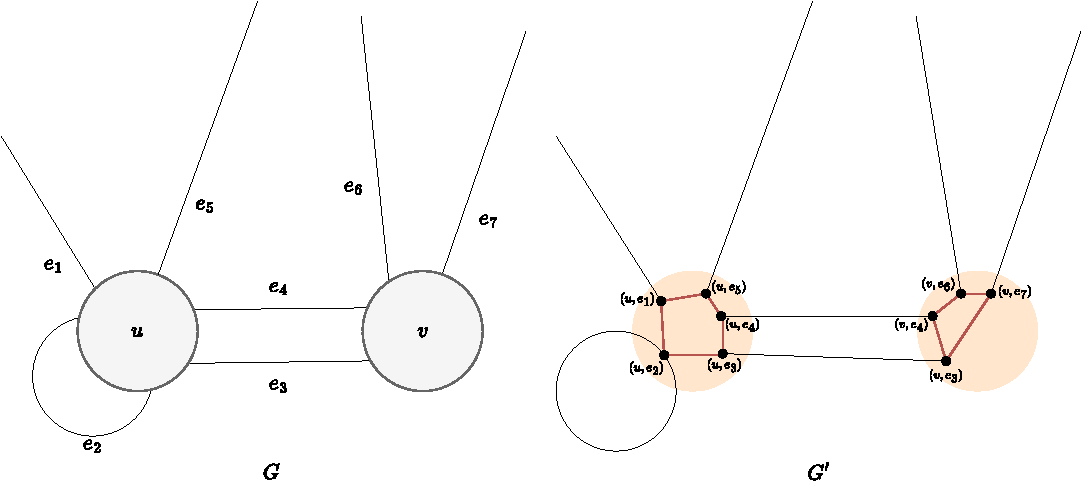
\includegraphics[width=\textwidth]{images/degree_reduction.pdf}
  \caption{次数削減変換の例. 橙色の内部の頂点集合がクラウドであり, クラウド内の辺は\cref{thm:construction-of-expander-graph}によって構成されるが, ここでは図の簡単のため$X_d$を長さ$d$の閉路としている. $G'$における黒い辺の制約は対応する元のグラフの辺と同一の制約とし, クラウド内の赤辺の制約は等式制約とする.}
  \label{fig:degree-reduction}
\end{figure}

元のグラフの各頂点$u\in V$に対し, 
\[[u]=\qty{ (u,e) \in \{u\}\times E \colon e=\{u,v\} \text{ for some } v\in V }\]
を(この証明のローカルな用語として)\emph{$u$-クラウド}と呼ぶことにする.
新しい頂点集合$V'$は$V'=\bigcup_{u\in V} [u]$である.
すなわち, $u$をそれに接続する辺の本数(自己ループは1個分としてカウント)だけコピーして得られる集合が$[u]$である.

次に辺集合$E'$を以下のように構成する.
まず, $(X_n)_{n\in\Nat}$を\cref{thm:construction-of-expander-graph}によって構成される$n$頂点$d_0$-正則$\lambda$-エクスパンダーの族とする.
元のグラフの各頂点$u\in V$に対し, $d=\abs{[u]}$としたとき, 頂点集合$[u]$上で$X_d$と同型なグラフを構成し, それを$([u],E_u)$とする.
このとき, 各$u$-クラウド内部の辺集合$E_{\mathrm{inner}}$は
\begin{align*}
  E_{\mathrm{inner}} = \bigcup_{u\in V} E_u
\end{align*}
とする.
次に異なるクラウド間を繋ぐ辺集合$E_{\mathrm{outer}}$を
\begin{align*}
  E_{\mathrm{outer}} = \qty{\qty{ (u,e), (v,e) } \colon e\notin [u]\cap[v]}
\end{align*}
とする.
このとき, グラフ$G'$の辺集合$E'$は
\begin{align*}
  E' = E_{\mathrm{inner}} \cup E_{\mathrm{outer}}
\end{align*}
となる.

次に各辺$e'\in E'$の制約$c'_{e'}$を以下のように定める:
\begin{itemize}
\item 辺$e'\in E_{\mathrm{outer}}$がクラウド間をつなぐ辺ならば, その制約は対応する元の辺$e$の制約と同じとする.
すなわち, $e'=\qty{ (u,e), (v,e) }$ならば, $c'_{e'}=c_e$である.
\item 辺$e'\in E_{\mathrm{inner}}$がクラウド内部の辺ならば, その制約を$c'_{e'}=\{(\sigma,\sigma)\colon \sigma\in\Sigma\}$, すなわち等式制約とする.
\end{itemize}

このようにして得られる制約グラフ$G'=\ip{(V',E'),\Sigma,\calC'}$が補題の主張を全て満たすことを確認する.
まず, $G'$は$(d_0+1)$-正則である.
実際, $G'$の各頂点$(u,e)\in V'$に接続する辺は, クラウド内の辺が$d_0$本, クラウド間の辺が$1$本である.
また, $G$から$G'$を構成する際に新たに追加する辺は$E_{\mathrm{inner}}$のみであり, これは高々$\sum_{u\in V}\frac{d_0\deg_G(u)}{2} \le d_0\abs{E}$本である (ここで\cref{eq:hand_shake_multigraph}を用いた).
従って
\begin{align}
  \abs{E'} = \abs{E_{\mathrm{inner}}} + \abs{E_{\mathrm{outer}}} \le \qty(d_0+1)\abs{E} \label{eq:bound_of_E'}
\end{align}
を満たす.
また, $V'$の要素数は次数の総和に等しいため, $\abs{V'}\le 2\abs{E}$を満たす.
次に, $\UNSAT(G)=0$ならば$\UNSAT(G')=0$である.
実際, 元の制約グラフの全ての制約を満たす割り当て$a\colon V\to\Sigma$に対し, $G'$の割り当て$a'\colon V'\to\Sigma$を
\begin{align*}
  a'(u,e) = a(u)
\end{align*}
と定めると, $a'$は$G'$の制約を満たす (同一クラウド内の頂点には全て同じ値が割り当てられるため, クラウド内の辺の制約は全て満たされ, クラウド間の辺に対応する制約は$a$の取り方により全て満たされることがわかる).

最後の主張, すなわち$\UNSAT(G') \ge c'\cdot \UNSAT(G)$となる定数$c'>0$が存在すること示す.
定数$c'>0$を
\begin{align}
  c' = \min\qty{\frac{(1-\lambda_0)d_0}{8(d_0+1)}, \frac{1}{2(d_0+1)}} \label{eq:c_of_degree_reduction}
\end{align}
と定める.
$\UNSAT(a';G')=\UNSAT(G')$を満たす割り当て$a'\colon V'\to\Sigma$を任意に取る.
この割り当て$a'$に対し, 元のグラフ$G$の割り当て$a\colon V\to\Sigma$を
\begin{align*}
  a(u) = \Maj((a'(u,e))_{(u,e) \in [u]})
\end{align*}
と定める. ここで$\Maj(\cdot)$は多数決関数であり,
タイは任意に選ぶとする.
例えば$\Maj(1,2,2)=2$, $\Maj(1,2,3,3)=3$, $\Maj(1,2,2,3,3)=2$である ($\Maj(1,2,2,3,3)=3$としても良いが, ここでは便宜上小さい方の数字を採用している).

以降, 割り当て$a'\colon V'\to\Sigma$に対し, 頂点$(u,e)\in V'$への割り当て$a'(u,e)$を頂点$(u,e)$の\emph{意見}と呼ぶこととする.
同様に, 割り当て$a\colon V\to\Sigma$に対し, 頂点$u\in V$への割り当て$a(u)$を頂点$u$の意見と呼ぶこととする.
直感的には頂点$u$の意見は対応する$u$-クラウド内の頂点の意見の多数決である.


辺集合$F\subseteq E$を割り当て$a$によって充足されない辺の集合, すなわち
\begin{align*}
  F = \qty{ e=\{u,v\}\in E \colon (a(u),a(v)) \not\in c_e}
\end{align*}
と定義する.
ここで$\calC = (c_e)_{e\in E}$は元の制約グラフ$G$の制約である.
同様に, $F'\subseteq E'$を割り当て$a'$によって充足されない辺の集合とする.
このとき$\UNSAT(a;G) = \frac{|F|}{|E|}$および$\UNSAT((a';G') = \frac{|F'|}{|E'|}$である.
頂点部分集合$S\subseteq V'$を$a$の多数決で選ばれなかった意見を持つ頂点の集合, すなわち
\begin{align*}
  S = \qty{ (u,e) \in V' \colon a(u) \ne a'(u,e)}
\end{align*}
と定義し, 各$v\in V$に対し$S^v = S\cap [v]$とし, 各$\sigma\in \Sigma$に対し$S^v_\sigma = \qty{ (u,e)\in S^v \colon a'(u,e)=\sigma }$とする (\cref{fig:majority-degree-reduction}).
なお, $\sigma\in\Sigma$が多数決の意見 (すなわち$\sigma=a(v)$)のとき, $S^v_\sigma=\emptyset$とする.

\begin{figure}[h]
  \centering
  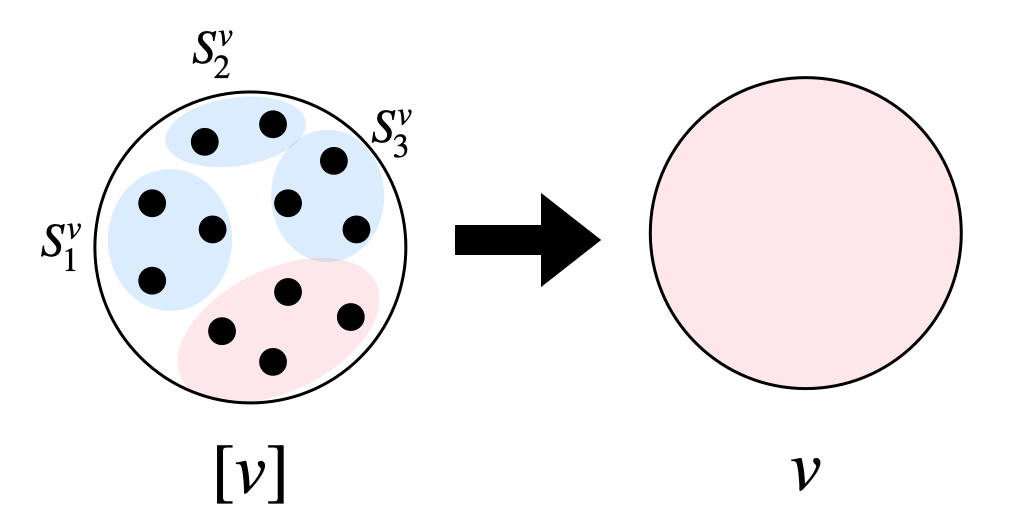
\includegraphics[width=\textwidth]{images/majority_degree_reduction.png}
  \caption{多数決によって選ばれなかった$v$-クラウド内の頂点の集合を$S_v\subseteq [v]$とする. \label{fig:majority-degree-reduction}}
\end{figure}

以下の二つのケースを考える:

\paragraph*{ケース1. $\abs{S} \ge \frac{\UNSAT(a;G)}{2}\abs{E}$の場合.}

各頂点$v\in V$と多数決によって選ばれなかった意見$\sigma\in\Sigma \setminus \{a(v)\}$に対し$\abs{S^v_\sigma} \le \frac{\abs{[v]}}{2}$である
(そうでなければ意見$\sigma$が多数決によって選ばれなかったことに矛盾する).
ここで$v$-クラウド内部のグラフは$d_0$-正則$\lambda_0$-エクスパンダーであるため, その頂点部分集合$S^v_\sigma\subseteq[v]$に対するエクスパンダー混交補題(\cref{lem:expander-mixing-lemma})より,
\begin{align*}
  W(S^v_\sigma, [v]\setminus S^v_\sigma) \ge (1-\lambda_0)\cdot \frac{d_0\abs{S^v_\sigma}}{2}
\end{align*}
となる. ここで$W(S,T)$は$v$-クラウド内部のグラフ$([v],E_v)$の辺であって$S$と$T$の間をまたがる辺の本数である.
ここで$S^v_\sigma$と$[v]\setminus S^v_\sigma$をまたがる全ての辺の両端点の意見は異なるため, $a'$はこれらの辺を充足しない. よってこれらの辺は全て$F'$に含まれる.
従って
\begin{align*}
  \abs{F'} &\ge \frac{1}{2}\sum_{v,\sigma} W(S^v_\sigma, [v]\setminus S^v_\sigma) \\
  &\ge \frac{(1-\lambda_0)d_0}{4}\sum_{v,\sigma} \abs{S^v_\sigma} \\
  &= \frac{(1-\lambda_0)d_0}{4}\abs{S} \\
  &\ge \frac{(1-\lambda_0)d_0}{8}\UNSAT(a;G)\cdot \abs{E}  & & \because \text{ケース1の仮定} \\
  &\ge \frac{(1-\lambda_0)d_0}{8(d_0+1)}\UNSAT(a;G)\cdot \abs{E'}. & & \because\text{\cref{eq:bound_of_E'}}
\end{align*}
特にこれから$\UNSAT(a';G') = \frac{\abs{F'}}{\abs{E'}}\ge \frac{(1-\lambda_0)d_0}{8(d_0+1)}\cdot\UNSAT(a;G)$が成り立つ.

\paragraph*{ケース2. $\abs{S} < \frac{\UNSAT(a;G)}{2}\abs{E}$の場合.}
任意の辺$e = \{u,v\} \in F$に対して, それに対応する$G'$の辺$e' = \{(u,e),(v,e)\}$を考える.
\begin{itemize}
\item もしも$a(u)=a'(u,e)$かつ$a(v)=a'(v,e)$が成り立つならば, $e'$と$e$は同じ制約を持ち, $e\in F$であることから$e'\in F'$である.
\item そうでない, すなわち$a(u)\ne a'(u,e)$または$a(v)\ne a'(v,e)$が成り立つならば, $(u,e)$と$(v,e)$のうち少なくとも一方はその意見が多数決として選ばれない, すなわち$(u,e)\in S$または$(v,e)\in S$が成り立つ.
\end{itemize}
以上より$\abs{F} \le \abs{F'} + \abs{S}$が成り立つので
\begin{align*}
  \abs{F'} &\ge \abs{F} - \abs{S} \\
  &\ge \abs{E}\UNSAT(a;G) - \frac{\UNSAT(a;G)}{2}\abs{E} & & \because \text{ケース2の仮定}\\
  &= \frac{\UNSAT(a;G)}{2}\abs{E} \\
  &\ge \frac{\UNSAT(a;G)}{2(d_0+1)}\abs{E'} & & \because\text{\cref{eq:bound_of_E'}}
\end{align*}
となり, これから
\begin{align*}
  \UNSAT(a';G') = \frac{\abs{F'}}{\abs{E'}} \ge \frac{1}{2(d_0+1)}\cdot \UNSAT(a;G)
\end{align*}
が成り立つ.

ケース1,2より, \cref{eq:c_of_degree_reduction}で定まる定数$c'>0$に対して$\UNSAT(a';G') \ge c'\cdot \UNSAT(a;G) \ge c'\cdot \UNSAT(G)$が成り立つ.
\end{proof}

\subsection{エクスパンダー化}

次に, 与えられた正則な制約グラフをエクスパンダーグラフに変換する補題を示す.

\begin{lemma}{エクスパンダー化補題}{expanderization}
ある定数$\lambda<1,d,d_0\in\Nat$および次を満たす多項式時間アルゴリズム$A$が存在する:
アルゴリズム$A$は入力として$d$-正則な制約グラフ$G = \ip{ (V,E), \Sigma, \calC }$
を受け取り, $(d+d_0+1)$-正則で全頂点が自己ループを持ち, さらに$\lambda$-エクスパンダーである制約グラフ $G' = \ip{ (V, E'), \Sigma, \calC' }$ を出力する.
さらに, この制約グラフ$G'$は$\UNSAT(G') = \frac{d}{d+d_0+1}\UNSAT(G)$を満たす.
\end{lemma}

\begin{proof}
入力として与えられた制約グラフを$G=\ip{(V,E),\Sigma,\calC}$とする.
変換は以下のようにして行われる:
\begin{enumerate}
\item まず, \cref{thm:construction-of-expander-graph}を用いて頂点集合$V$上$d_0$-正則$\lambda_0$-エクスパンダーグラフを構成し, その辺集合を$E$に追加する (この際多重辺も許す).
\item 次に, 各頂点に自己ループを付与する.
\item ステップ1,2で追加した辺$e$に対応する制約$c'_e$を自明な制約$c'_e=\Sigma^2$とする.
\end{enumerate}
このようにして得られる制約グラフを$G'=\ip{(V',E'),\Sigma,\calC'}$とする.
元の制約グラフ$G$が$d$-正則であることから, $G'$は$(d+d_0+1)$-正則である (自己ループの次数への寄与は$1$であることに注意).
また, ステップ2より$G'$は全頂点が自己ループを持つ.

次に$\UNSAT(G')=\frac{d}{d+d_0+1}\UNSAT(G)$を示す.
任意の割り当て$a\colon V \to \Sigma$に対し, 
ステップ1,2で追加した辺に対応する制約は常に充足されるため, 両者が充足\emph{しない}制約の個数は一致する.
すなわち$\abs{E}\UNSAT(a;G) = \abs{E'}\UNSAT(a;G')$が成り立つので
\begin{align*}
  \UNSAT(G') = \min_{a}\UNSAT(a;G') = \frac{\abs{E}}{\abs{E'}}\min_a \UNSAT(a;G) = \frac{d}{d+d_0+1}\UNSAT(G)
\end{align*}
が成り立つ.

最後に$G'$が$\lambda:=\frac{d}{d+d_0+1}+\frac{\lambda_0(d_0+1)}{d+d_0+1}$に対し$\lambda$-エクスパンダーであることを示す.
元のグラフ$G$の遷移確率行列を$P\in[0,1]^{V\times V}$とし,
ステップ1,2で追加した辺からなるグラフを$G_0$とし, その遷移確率行列を$P_0\in[0,1]^{V\times V}$とする.
また, 最終的に得られるグラフ$G'$の遷移確率行列を$P'\in[0,1]^{V\times V}$とする.
元のグラフ$G$は$d$-正則, 追加したグラフ$G_0$は$(d_0+1)$-正則であるため
\begin{align*}
  P' = \frac{d}{d+d_0+1}P + \frac{d_0+1}{d+d_0+1}P_0
\end{align*}
となる.
さらに$P_0$は$\lambda_0$-エクスパンダーであるため, 全成分$1$のベクトル$\allone$と直交する任意のベクトル$x\in \Real^V$に対し
\begin{align*}
  x^\top P' x &= \frac{d}{d+d_0+1}x^\top P x + \frac{d_0+1}{d+d_0+1}x^\top P_0 x \\
  &\ge \frac{d}{d+d_0+1}\norm{x}^2 + \frac{d_0+1}{d+d_0+1}\lambda_0\norm{x}^2 & & \because\text{$P_0$のエクスパンダー性}\\
  &\le \qty( \frac{d}{d+d_0+1} + \frac{\lambda_0(d_0+1)}{d+d_0+1} )\norm{x}^2
\end{align*}
より, $\lambda(P')\le \frac{d}{d+d_0+1} + \frac{\lambda_0(d_0+1)}{d+d_0+1}$が成り立つ.
\end{proof}

これにより\cref{lem:constant-degree-expanderization}を示す準備が整った.
\begin{proof}[\cref{lem:constant-degree-expanderization}の証明]

与えられた制約グラフ$G$に対し, まず$G$を入力として\cref{lem:degree-reduction}のアルゴリズムを実行し, その出力を$G_1$とする.
この制約グラフ$G_1$は\cref{lem:degree-reduction}の主張より, $d$-正則である.
次に, $G_1$を入力として\cref{lem:expanderization}のアルゴリズムを実行し, その出力を最終的な出力$G$とする.
この制約グラフ$G'$は\cref{lem:expanderization}の主張より, 全頂点が自己ループを持ち, $(d+d_0+1)$-正則かつ$\lambda$-エクスパンダーである.
また, この一連の変換によって$\size(G')$は$\size(G)$の定数倍にしかならない.

最後に$\UNSAT$の値を考える.
元の制約グラフ$G$が$\UNSAT(G)=0$ならば, \cref{lem:degree-reduction,lem:expanderization}より
$\UNSAT(G') = \frac{d}{d+d_0+1}\UNSAT(G_1) = 0$を得る.
一方で
\begin{align*}
  \UNSAT(G') = \frac{d}{d+d_0+1}\UNSAT(G_1) \ge \frac{d}{d+d_0+1}\cdot c'\cdot\UNSAT(G).
\end{align*}
すなわち$\beta = \frac{d}{d+d_0+1}\cdot c'$に対して主張が成り立つことが示された.
\end{proof}

\section{制約グラフのべき乗}

\cref{lem:constant-degree-expanderization}により, 任意の制約グラフを定数次数エクスパンダーに変換することができる.
この節では, そのような制約グラフに対し, 以下で定義する\emph{べき乗}という操作を考えることで, その$\UNSAT$の値を増幅させることができることを示す.

\begin{definition}{制約グラフの冪乗}{power-of-constraint-graph}
  パラメータ$t\in\Nat$および全頂点が自己ループを持つ$d$-正則な制約グラフ$G=\ip{(V,E),\Sigma,\calC}$に対し, べき乗$G^t = \ip{(V,\boldE),\Sigma^{\ceil{t/2}},\calC^t}$を, 以下のようにして定義する:
  \begin{itemize}
    \item 頂点集合は同じ$V$とする.
    \item 二頂点$u,v\in V$に対し, 長さ$t$の$uv$-路の個数と同じだけ$uv$間に多重辺を用意する. このようにして得られる辺の多重集合を$\boldE$とし, その元を$\bolde = \{u,v\} \in \boldE$とする.
    \item アルファベット集合は$\Sigma^{d^{\ceil{t/2}}}$とする. ここで, 頂点$u$に意見$\sigma=(\sigma_1,\dots,\sigma_{d^{\ceil{t/2}}}) \in \Sigma^{d^{\ceil{t/2}}}$が割り当てられたとき, 次の意味を持つ: 元の$d$-正則グラフ$G$上で頂点$u$から距離$\ceil{t/2}$以内の頂点の集合を$\Gamma(u)$とし, その元を頂点番号の大小順で並べて$\Gamma(u)=\qty{ v_1,\dots,v_\ell}$ とする (ここで$G$の$d$-正則性より$\ell \le d^{\ceil{t/2}}$である). このとき, 意見$\sigma$は$v_1,\dots,v_\ell$の各頂点に$\Sigma$の元を割り当てる関数$\sigma \colon \Gamma(u)\to\Sigma$とみなす.
    \begin{itemize}
      \item 例えば$\ell < d^{\ceil{t/2}}$の場合は相異なる二つの$\sigma,\sigma'\in\Sigma$が同一の関数を与えることもある.
      \item 頂点$u$と$\sigma\in\Sigma^{\ceil{t/2}}$の取り方によっては同一の頂点に対し, 相異なる$\Sigma$の元を割り当てるため$\sigma\in\Sigma^{\ceil{t/2}}$を関数$\Gamma(u)\to\Sigma$とみなせない場合もある. このようなとき, 意見$\sigma$は$u$にとって\emph{不適切}といい, 不適切でない場合は\emph{適切}であるという.
    \end{itemize}
    \item 辺$\bolde = \{u,v\} \in \boldE$ に対応する制約$\boldc_{\bolde}\in \calC^t$は次の二つを満たす割り当て$(\sigma,\sigma')\in \Sigma^{d^{\ceil{t/2}}} \times \Sigma^{d^{\ceil{t/2}}}$によって満たされる:
    \begin{itemize}
      \item 意見$\sigma$と$\sigma'$はそれぞれ$u,v$にとって適切であり, これらの意見は関数$\sigma\colon \Gamma(u)\to\Sigma$と$\sigma'\colon \Gamma(v)\to\Sigma$と同一視できる.
      \item 全ての頂点$a\in \Gamma(u)\cap \Gamma(v)$に対し, $\sigma(a)=\sigma'(a)$が成り立つ.
      \item 一方の端点が$\Gamma(u)$, もう一方の端点が$\Gamma(v)$に属する全ての辺$e=\{s,t\}\in E$に対し, $(\sigma(s), \sigma'(t))\in c_e$が成り立つ.
    \end{itemize}
  \end{itemize}
\end{definition}

\begin{lemma}{べき乗の性質}{property-of-power}
  ある定数$\beta=\beta(\lambda,d,\abs{\Sigma})$が存在して以下が成り立つ:
  パラメータ$t\in\Nat$および全頂点が自己ループを持つ$d$-正則な制約グラフ$G=\ip{(V,E),\Sigma,\calC}$に対し, べき乗$G^t = \ip{(V,\boldE),\Sigma^{\ceil{t/2}},\calC^t}$を, \cref{def:power-of-constraint-graph}で定義する.
  このとき
  \begin{itemize}
    \item 元の制約グラフ$G$が$\lambda$-エクスパンダーであるとき, $G^t$は$d^t$-正則$\lambda^t$-エクスパンダーである.
    \item $\size(G^t) \le \size(G)\cdot d^t$である.
    \item $\UNSAT(G)=0$ならば$\UNSAT(G^t)=0$である.
    \item $\UNSAT(G^t) \ge \beta\sqrt{t}\cdot \min\qty{ \UNSAT(G), \frac{1}{t} }$である.
  \end{itemize}
\end{lemma}
\begin{proof}

\cref{lem:power-of-regular-expander}により, $G$が$d$-正則かつ$\lambda$-エクスパンダーならば$G^t$は$d^t$-正則かつ$\lambda^t$-エクスパンダーとなる.
特に, $\size(G^t) \le \size(G)\cdot d^t$である.

また, $\UNSAT(G)=0$ならば, 全制約を満たす割り当て$a\colon V \to \Sigma$を用いて$G^t$の全ての制約を満たす割り当て$a'\colon V \to \Sigma^{\ceil{t/2}}$を, 各頂点$u\in V$の適切な意見$a'(u)\colon\Gamma(U)\to\Sigma$を
\begin{align*}
  a'(u)\colon s \mapsto a(s)
\end{align*}
と定めることによって得られる.
すなわち$\UNSAT(G^t)=0$である.

最後に$\UNSAT(G^t)$の下界を証明する.


\end{proof}

\section{アルファベット削減}



